\documentclass[border=8pt]{standalone}
\usepackage{mathpazo}
\usepackage{tikz}
\usetikzlibrary{arrows.meta}

\definecolor{stblue}{HTML}{7B97AD}
\definecolor{rwgold}{HTML}{B8995E}
\definecolor{sage}{HTML}{7A9A7E}
\definecolor{terracotta}{HTML}{C47A6A}
\definecolor{dkbrown}{HTML}{3D3530}
\definecolor{wmgray}{HTML}{7B7067}
\definecolor{lavender}{HTML}{907EA0}
\definecolor{goldfill}{HTML}{F5EFE4}
\definecolor{bluefill}{HTML}{E8EDF2}
\definecolor{sagefill}{HTML}{E8F0E9}
\definecolor{lavfill}{HTML}{EDE8F0}
\definecolor{terrafill}{HTML}{F2E6E3}

\begin{document}
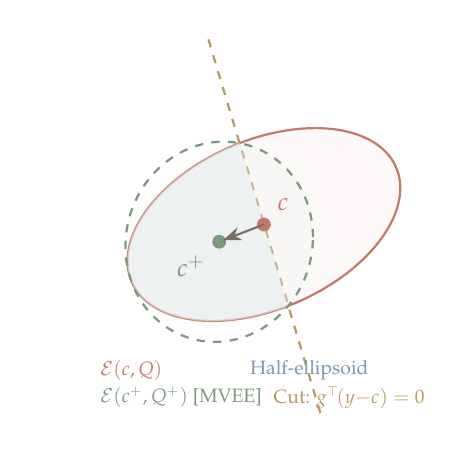
\begin{tikzpicture}[>=Stealth]

% Original ellipsoid: c=(0,0), L=[[1.73205081,0],[0.46188022,1.1343133]]
% x(t) = 1.732*cos(t), y(t) = 0.462*cos(t) + 1.134*sin(t)
% Q = LL^T = [[3, 0.8],[0.8, 1.5]] approximately

% Draw original ellipsoid
\draw[terracotta, thick, fill=terrafill, fill opacity=0.25]
  plot[domain=0:360, samples=200, smooth]
  ({1.732*cos(\x)}, {0.462*cos(\x) + 1.134*sin(\x)});

% Cut direction: g_normalized = (0.958, 0.287)
% Hyperplane g^T y = 0: passes through origin, perpendicular to g
% Line direction: (-0.287, 0.958)
% Draw cutting hyperplane
\draw[rwgold, thick, dashed] ({-2.5*(-0.287)}, {-2.5*0.958}) -- ({2.5*(-0.287)}, {2.5*0.958});

% Shade the half-ellipsoid (g^T y <= 0 side)
% We clip to the half-plane g^T y <= 0
\begin{scope}
  \clip ({2.5*(-0.287)}, {2.5*0.958}) -- ({-2.5*(-0.287)}, {-2.5*0.958})
        -- (-3, -2.5) -- (-3, 2.5) -- cycle;
  \fill[bluefill, opacity=0.6]
    plot[domain=0:360, samples=200, smooth]
    ({1.732*cos(\x)}, {0.462*cos(\x) + 1.134*sin(\x)});
\end{scope}

% New ellipsoid (MVEE): c_new=(-0.568, -0.219)
% L_new=[[1.191,0],[0.059,1.270]]
\draw[sage, thick, dashed, fill=sagefill, fill opacity=0.15]
  plot[domain=0:360, samples=200, smooth]
  ({1.191*cos(\x) + (-0.568)}, {0.059*cos(\x) + 1.270*sin(\x) + (-0.219)});

% Original center
\fill[terracotta] (0,0) circle (2.5pt);
\node[terracotta, font=\small, above right] at (0.05, 0.05) {$c$};

% New center
\fill[sage] (-0.568, -0.219) circle (2.5pt);
\node[sage, font=\small, below left] at (-0.62, -0.27) {$c^+$};

% Arrow from c to c+
\draw[->, wmgray, thick] (0,0) -- (-0.52, -0.20);

% Legend
\node[terracotta, font=\scriptsize, right] at (-2.2, -1.85) {$\mathcal{E}(c, Q)$};
\node[stblue, font=\scriptsize, right] at (-0.3, -1.85) {Half-ellipsoid};
\node[rwgold, font=\scriptsize, right] at (0.0, -2.2) {Cut: $g^\top\!(y{-}c)=0$};
\node[sage, font=\scriptsize, right] at (-2.2, -2.2) {$\mathcal{E}(c^+, Q^+)$ [MVEE]};

\end{tikzpicture}
\end{document}
